\myChapter{\'Etat de l'art sur la pr\'ediction des contaminants \'emergents de l'eau par intelligence artificielle}{\'Etat de l'art}
\label{chap:etat-art}
\myMiniToc{section}{Sommaire}

% =========================================================
\mySection{Introduction}{}
\label{sec:intro-chap2}
% =========================================================

La surveillance des PFAS dans les eaux souterraines constitue un d\'efi analytique et \'economique~: une analyse par chromatographie liquide coupl\'ee \`a la spectrom\'etrie de masse tandem co\^ute plusieurs centaines d'euros par \'echantillon, alors que les seuils r\'eglementaires se durcissent (4~ng/L pour le PFOA et le PFOS depuis 2023 aux \'Etats-Unis~\cite{epa2023npdwr}, 0,5~$\mu$g/L pour la somme des PFAS dans la directive europ\'eenne 2020/2184~\cite{eu2020drinkingwater}).
Un contr\^ole exhaustif du parc de puits \'etant hors de port\'ee de la plupart des gestionnaires, les m\'ethodes d'intelligence artificielle se sont impos\'ees comme outils de priorisation~: orienter les campagnes vers les sites \`a plus forte probabilit\'e de d\'epassement, \`a partir d'informations contextuelles disponibles sans analyse PFAS pr\'ealable.
Les enjeux sanitaires, la chimie des PFAS et les fondements algorithmiques mobilis\'es ayant \'et\'e d\'etaill\'es au chapitre~\ref{chap:generalites}, ce chapitre se concentre sur leur application \`a la surveillance.

Depuis la d\'ecennie 2010, deux g\'en\'erations de m\'ethodes sont bien document\'ees, une troisi\`eme \'etant en cours de constitution.
La premi\`ere repose sur des mod\`eles probabilistes et tabulaires (r\'eseaux bay\'esiens, for\^ets al\'eatoires, gradient boosting) traitant chaque puits comme un vecteur de descripteurs ind\'ependants.
La deuxi\`eme introduit des architectures plus complexes~: d'abord des r\'eseaux de neurones sur donn\'ees mol\'eculaires (QSAR), puis des cha\^ines de classifieurs semi-supervis\'ees pr\'edisant simultan\'ement plusieurs dizaines d'analytes.
La troisi\`eme, encore embryonnaire dans la litt\'erature PFAS publi\'ee, mobilise les graphes h\'et\'erog\`enes pour encoder explicitement la topologie du r\'eseau de surveillance~; aucune \'etude ne l'a syst\'ematiquement valid\'ee sur ce type de donn\'ees.

Ce chapitre examine ces deux g\'en\'erations et la direction \'emergente de mani\`ere structur\'ee~: le cadre conceptuel de la revue (section~\ref{sec:chap2-cadre}), dont la distinction mode pr\'edictif/confirmatoire (section~\ref{sec:chap2-modes})~; les m\'ethodes tabulaires, probabilistes, d'ensemble et d'attribution de sources (section~\ref{sec:chap2-tabulaire})~; les architectures profondes et relationnelles (section~\ref{sec:chap2-deep})~; une discussion transversale (section~\ref{sec:chap2-discussion}) assortie des lacunes structurelles (section~\ref{sec:chap2-lacunes})~; enfin une synth\`ese (section~\ref{sec:synthese-chap2}).


% =========================================================
\mySection{Cadre conceptuel de la revue}{}
\label{sec:chap2-cadre}
% =========================================================

Avant d'examiner les travaux, cinq \'el\'ements conceptuels propres \`a cette revue doivent \^etre pos\'es.
Le premier est la formalisation du probl\`eme de pr\'ediction ML sur donn\'ees PFAS.
Le deuxi\`eme relie la s\'election des variables contextuelles aux m\'ecanismes physico-chimiques de transport des PFAS, fondement commun \`a toutes les \'etudes examin\'ees.
Le troisi\`eme et le quatri\`eme \'etablissent le socle m\'etrique commun (m\'etriques d'\'evaluation, gestion du d\'es\'equilibre de classes) qui sert de r\'ef\'erence \`a toutes les comparaisons inter-\'etudes.
Le cinqui\`eme, et le plus fondamental, est la distinction entre mode pr\'edictif et mode confirmatoire~: mal comprise, elle conduit \`a des comparaisons de performance trompeuses entre \'etudes.


\mySubSection{Formalisation du probl\`eme de pr\'ediction PFAS par apprentissage automatique}{}
\label{sec:chap2-formalisation}

La pr\'ediction du statut de contamination d'un puits par apprentissage automatique revient \`a estimer une fonction $g : \mathcal{X} \rightarrow \mathcal{Y}$ associant \`a chaque puits, d\'ecrit par un vecteur de variables $\mathbf{x} \in \mathcal{X}$, une cible $y \in \mathcal{Y}$.
Le vecteur $\mathbf{x}$ rassemble les descripteurs disponibles (g\'eologie, hydrologie, proximit\'e aux sources, qualit\'e g\'en\'erale de l'eau)~; sa composition, avec ou sans concentrations PFAS mesur\'ees, d\'etermine le r\'egime d'\'evaluation discut\'e en section~\ref{sec:chap2-modes}.
La fonction $g$ est ajust\'ee sur un jeu d'entra\^inement \'etiquet\'e en minimisant une fonction de perte, puis \'evalu\'ee sur des donn\'ees non vues (section~\ref{sec:ml-supervise}).

Les travaux examin\'es se distinguent par la nature de la cible $\mathcal{Y}$, qui commande le choix des m\'ethodes et des m\'etriques.
\begin{itemize}
    \item \emph{Classification binaire} ($y \in \{0,1\}$)~: pr\'esence ou absence d'un analyte, ou d\'epassement d'un seuil r\'eglementaire. C'est la formulation la plus r\'epandue (George et Dixit, Tokranov, Li et MacDonald Gibson, ainsi que le criblage total de Dong et al.).
    \item \emph{Classification multi-\'etiquettes} ($\mathbf{y} \in \{0,1\}^L$, $L$ analytes)~: pr\'ediction simultan\'ee de plusieurs dizaines d'analytes. Absente du cadre multiclasse classique pr\'esent\'e au chapitre~\ref{chap:generalites}, elle est propre \`a la litt\'erature PFAS~\cite{dong2024pfas} et conditionne le choix des architectures pr\'esent\'ees en section~\ref{sec:chap2-semisup}.
    \item \emph{Cartographie de vuln\'erabilit\'e} ($y$ continu ou ordinal)~: production d'un score de risque r\'egional ou national plut\^ot que d'une \'etiquette par puits (Hu et al., McMahon et al.).
\end{itemize}

Deux propri\'et\'es traversent ces formulations.
D'une part, la cible binaire d\'epend d'un seuil qui a \'evolu\'e avec la r\'eglementation, ce qui complique la comparaison directe des performances entre \'etudes anciennes et r\'ecentes (section~\ref{sec:chap2-modes}).
D'autre part, le d\'es\'equilibre structurel de classes (section~\ref{sec:chap2-desequilibre}, avec SMOTE~\cite{chawla2002smote} et ADASYN~\cite{he2008adasyn}) est particuli\`erement marqu\'e dans les corpus PFAS, le rapport entre classe minoritaire et classe majoritaire s'\'etalant de 1/10 \`a 1/50~\cite{dong2024pfas}~; le score F1 (section~\ref{sec:chap2-metriques}) sert d'indicateur de r\'ef\'erence, compl\'et\'e par la ROC-AUC pour les comparaisons inter-\'etudes.

\mySubSection{M\'ecanismes de transport des PFAS et pertinence des variables contextuelles}{}
\label{sec:chap2-transport}

La s\'election des variables contextuelles dans les mod\`eles ML de pr\'ediction des PFAS n'est pas arbitraire~: elle d\'ecoule directement des m\'ecanismes physico-chimiques qui gouvernent le devenir et le transport des PFAS en milieu souterrain.
Trois processus principaux, d\'ecrits par Guelfo et al.~\cite{guelfo2021pfas} dans une revue exhaustive de l'\'etat de la science, conditionnent la distribution spatiale des concentrations observ\'ees.

\paragraph{Advection et att\'enuation en fonction de la distance.}
Les PFAS se d\'eplacent principalement par advection avec le flux d'eau souterraine, suivant les lignes d'\'ecoulement depuis les zones de recharge vers les zones de d\'echarge.
Prevedouros et al.~\cite{prevedouros2006pfas} montrent que les concentrations de PFCAs d\'ecroissent avec la distance aux sources ponctuelles~: la proximit\'e \`a une installation fluorochimique, une base militaire (usage de mousses AFFF) ou une station d'\'epuration constitue donc un proxy du flux de contamination advectif.
C'est ce constat m\'ecaniste qui fonde l'utilisation syst\'ematique, dans toutes les \'etudes examin\'ees, du nombre d'installations \`a 1, 3, 10 et 50~km comme variables pr\'edictives.

\paragraph{R\'etention sur la matrice solide.}
Brusseau et al.~\cite{brusseau2019pfas} \'etablissent un mod\`ele de r\'etention complet montrant que les PFAS se sorbent sur la mati\`ere organique du sol et sur les interfaces air-eau des zones vadoses~: la granulom\'etrie (proportion d'argiles, de limons, uniformit\'e de la distribution), la teneur en mati\`ere organique et la profondeur de la nappe modulent fortement la mobilit\'e des diff\'erentes familles de PFAS.
Les compos\'es \`a longue cha\^ine (PFOS, PFOA) se retiennent davantage que les compos\'es \`a cha\^ine courte (PFBS, PFPeA), plus mobiles mais aussi plus difficiles \`a \'eliminer.
Ce m\'ecanisme justifie l'inclusion de descripteurs de sol (granulom\'etrie, teneur en argile, ratio eau-argile) dans les vecteurs de features des mod\`eles tabulaires.

\paragraph{D\'eposition atmosph\'erique.}
Les PFAS volatils ou semi-volatils (fluorot\'elom\`eres, sulfonamides) sont \'emis dans l'atmosph\`ere par les installations industrielles, transport\'es sur des distances pouvant d\'epasser 50~km et d\'epos\'es par les pr\'ecipitations~\cite{guelfo2021pfas}.
Ce vecteur de contamination diffus et longue port\'ee explique pourquoi les variables m\'et\'eorologiques (humidit\'e, pr\'ecipitations, qualit\'e de l'air~: PM$_{2,5}$, NO$_2$) figurent parmi les pr\'edicteurs importants identifi\'es par Dong et al.~\cite{dong2024pfas}, alors qu'elles ne sont pas directement li\'ees aux sources ponctuelles locales.

\paragraph{Cons\'equences pour la mod\'elisation par graphes.}
L'advection cr\'ee une d\'ependance spatiale structurelle entre puits~: deux puits situ\'es en aval d'une m\^eme source partagent un contexte de contamination commun qui ne peut pas \^etre captur\'e par des vecteurs ind\'ependants.
Cette d\'ependance est directionnelle (orient\'ee par le sens de l'\'ecoulement) et h\'et\'erog\`ene (fonction de l'intensit\'e du flux, de la lithologie, de la proximit\'e \`a la source).
Les graphes h\'et\'erog\`enes, et en particulier le Heterogeneous Graph Transformer~\cite{hu2020hgt}, sont con\c{c}us pour encoder cette topologie~: des n\oe uds de types distincts (puits de surveillance, installations sources, clusters g\'eographiques) sont reli\'es par des ar\^etes typ\'ees repr\'esentant la proximit\'e aux sources et le voisinage spatial, le long desquelles l'information de contamination se propage.
Cette justification m\'ecaniste fonde l'int\'er\^et des architectures relationnelles, discut\'ees comme direction \'emergente dans la lacune~L1 (section~\ref{sec:chap2-lacunes})~: la topologie d'\'ecoulement y est encod\'ee explicitement plut\^ot que d\'eduite de variables ind\'ependantes.


\mySubSection{M\'etriques d'\'evaluation des classifieurs de contamination PFAS}{}
\label{sec:chap2-metriques}

La comparaison des m\'ethodes exig\'ee par la revue n\'ecessite un socle m\'etrique commun, d'autant que les \'etudes examin\'ees ne rapportent pas toutes les m\^emes indicateurs.
Cette section fixe les d\'efinitions retenues pour la classification binaire (pr\'esence/absence d'un PFAS, d\'epassement d'un seuil r\'eglementaire), puis pr\'ecise le passage au cas multi-\'etiquettes~; Sokolova et Lapalme~\cite{sokolova2009metrics} en proposent l'analyse syst\'ematique dont nous reprenons l'ossature.
Toutes les m\'etriques d\'erivent de la \textbf{matrice de confusion} (tableau~\ref{tab:confusion}), qui recense quatre effectifs en confrontant les pr\'edictions \`a la v\'erit\'e terrain~: vrais positifs (VP), vrais n\'egatifs (VN), faux positifs (FP) et faux n\'egatifs (FN).

\begin{table}[H]
    \centering
    \caption{Matrice de confusion pour une classification binaire (classe positive~= site contamin\'e).}
    \label{tab:confusion}
    \begin{tabular}{lcc}
        \hline
        & Pr\'edit 0 & Pr\'edit 1 \\
        \hline
        R\'eel 0 & Vrai n\'egatif (VN) & Faux positif (FP) \\
        R\'eel 1 & Faux n\'egatif (FN) & Vrai positif (VP) \\
        \hline
    \end{tabular}
\end{table}

Le choix de l'indicateur n'est pas neutre en surveillance environnementale~: un faux n\'egatif (site contamin\'e non d\'etect\'e) expose une population, l\`a o\`u un faux positif (pr\'el\`evement inutile) n'entra\^ine qu'un co\^ut analytique.
Les m\'etriques sensibles aux faux n\'egatifs sont donc privil\'egi\'ees.

\paragraph{Exactitude.}
L'exactitude $\mathrm{Acc} = (VP+VN)/(VP+VN+FP+FN)$ mesure la proportion de pr\'edictions correctes.
Sous un fort d\'es\'equilibre de classes (section~\ref{sec:chap2-desequilibre}), elle devient trompeuse~: un classifieur pr\'edisant toujours la classe majoritaire atteint une exactitude proche de 1 sans d\'etecter le moindre site contamin\'e.

\paragraph{Pr\'ecision, rappel et sp\'ecificit\'e.}
Trois quantit\'es se lisent directement dans la matrice~:
\begin{equation}
    \text{Pr\'ecision} = \frac{VP}{VP + FP}, \qquad
    \text{Rappel} = \frac{VP}{VP + FN}, \qquad
    \text{Sp\'ecificit\'e} = \frac{VN}{VN + FP}.
    \label{eq:precision-rappel}
\end{equation}
La pr\'ecision indique, parmi les sites signal\'es contamin\'es, la part qui l'est r\'eellement.
Le rappel (ou sensibilit\'e) indique, parmi les sites r\'eellement contamin\'es, la part d\'etect\'ee~; en priorisation PFAS, il prime, puisque manquer un site pollu\'e est l'erreur la plus co\^uteuse.
La sp\'ecificit\'e indique, parmi les sites r\'eellement non contamin\'es, la part correctement \'ecart\'ee (taux de vrais n\'egatifs).
Son compl\'ement $1 - \text{Sp\'ecificit\'e}$, le taux de faux positifs, constitue l'abscisse de la courbe ROC.

\paragraph{Score F1 et $F_\beta$.}
Le score F1, moyenne harmonique de la pr\'ecision et du rappel, condense ces deux quantit\'es~:
\begin{equation}
    F_1 = 2 \cdot \frac{\text{Pr\'ecision} \times \text{Rappel}}{\text{Pr\'ecision} + \text{Rappel}}.
    \label{eq:f1}
\end{equation}
Sa g\'en\'eralisation $F_\beta = (1+\beta^2)\,\dfrac{\text{Pr\'ecision} \cdot \text{Rappel}}{\beta^2\,\text{Pr\'ecision} + \text{Rappel}}$ pond\`ere le rappel par un facteur $\beta$~; choisir $\beta > 1$ p\'enalise davantage les faux n\'egatifs, conform\'ement \`a la logique de surveillance.
La moyenne harmonique chute d\`es que la pr\'ecision ou le rappel est faible, ce qui rend le F1 plus exigeant que l'exactitude sous d\'es\'equilibre~\cite{sokolova2009metrics}.

\paragraph{Coefficient de corr\'elation de Matthews.}
Le coefficient de Matthews (MCC) combine les quatre cases de la matrice~:
\begin{equation}
    \mathrm{MCC} = \frac{VP \cdot VN - FP \cdot FN}{\sqrt{(VP+FP)(VP+FN)(VN+FP)(VN+FN)}}.
    \label{eq:mcc}
\end{equation}
Born\'e entre $-1$ et $+1$, il n'est \'elev\'e que si le classifieur r\'eussit simultan\'ement sur les deux classes.
Chicco et Jurman~\cite{chicco2020mcc} montrent qu'il reste plus fiable que le F1 et l'exactitude sous fort d\'es\'equilibre, car aucune classe ne peut \`a elle seule le gonfler.

\paragraph{Courbes ROC et pr\'ecision-rappel.}
La courbe ROC trace le taux de vrais positifs contre le taux de faux positifs \`a mesure que varie le seuil de d\'ecision~; son aire (\textbf{ROC-AUC}) quantifie la s\'eparabilit\'e des classes ind\'ependamment du seuil op\'erationnel~\cite{fawcett2006roc}.
Sous d\'es\'equilibre marqu\'e, cette aire peut para\^itre optimiste~; la courbe pr\'ecision-rappel et son aire (PR-AUC) refl\`etent alors plus fid\`element la performance sur la classe positive rare~\cite{davis2006prroc,saito2015prc}.

\paragraph{Choix retenu pour la revue.}
Le F1 sert d'indicateur de r\'ef\'erence pour les comparaisons inter-\'etudes, compl\'et\'e par la ROC-AUC lorsqu'elle est rapport\'ee.
En classification multi-\'etiquettes ($L$ analytes), le \textbf{F1 macro}, moyenne uniforme sur les $L$ analytes, est privil\'egi\'e~: il accorde le m\^eme poids \`a chaque analyte et \'evite de masquer les mauvaises performances sur les compos\'es rares, contrairement au F1 micro que dominent les analytes fr\'equents~\cite{sokolova2009metrics}.


\mySubSection{D\'es\'equilibre de classes et r\'e\'echantillonnage synth\'etique}{}
\label{sec:chap2-desequilibre}

Dans les corpus de surveillance PFAS, la classe positive (d\'etection ou d\'epassement de seuil) est structurellement minoritaire~: le rapport entre classe minoritaire et classe majoritaire peut atteindre 1/10 \`a 1/50 selon les analytes et la r\'egion~\cite{dong2024pfas,george2021pfas}.
Un classifieur entra\^in\'e sans correction tend alors \`a ignorer la classe positive pour maximiser l'exactitude globale, comportement inacceptable en surveillance sanitaire o\`u c'est pr\'ecis\'ement cette classe qui importe.
He et Garcia~\cite{he2009imbalanced} distinguent quatre familles de r\'eponses, souvent combin\'ees.

\paragraph{R\'e\'echantillonnage.}
La premi\`ere agit sur la distribution du jeu d'entra\^inement, par sous-\'echantillonnage de la classe majoritaire ou sur-\'echantillonnage de la classe minoritaire.
Le sur-\'echantillonnage al\'eatoire duplique des exemples existants, au risque du surapprentissage~; SMOTE et ADASYN, dominants dans la litt\'erature PFAS, g\'en\`erent au contraire des exemples synth\'etiques.
\textbf{SMOTE} (\emph{Synthetic Minority Over-sampling Technique})~\cite{chawla2002smote} interpole lin\'eairement entre un exemple $\mathbf{x}_i$ et l'un de ses $k$ plus proches voisins minoritaires~:
\begin{equation}
    \mathbf{x}_{\mathrm{new}} = \mathbf{x}_i + \lambda\,(\mathbf{x}_j - \mathbf{x}_i), \quad \lambda \sim \mathcal{U}(0,1).
    \label{eq:smote}
\end{equation}
\textbf{ADASYN} (\emph{Adaptive Synthetic Sampling})~\cite{he2008adasyn} concentre la g\'en\'eration pr\`es de la fronti\`ere de d\'ecision~: le nombre d'exemples allou\'e \`a chaque $\mathbf{x}_i$ cro\^it avec la fraction $r_i = \Delta_i/k$ de ses $k$ voisins appartenant \`a la classe majoritaire.
Cette focalisation adaptative est pertinente lorsque les sites contamin\'es sont spatialement dispers\'es dans un corpus h\'et\'erog\`ene, comme dans les \'etudes californiennes \`a grande \'echelle.

\paragraph{Pond\'eration du co\^ut.}
La deuxi\`eme famille conserve la distribution mais p\'enalise davantage les erreurs sur la classe minoritaire, en pond\'erant la fonction de perte par l'inverse de la fr\'equence des classes.
Native dans la plupart des impl\'ementations d'arbres d'ensemble via un param\`etre de poids de classe, elle \'evite la cr\'eation d'exemples artificiels.

\paragraph{Ajustement du seuil et m\'etriques adapt\'ees.}
La troisi\`eme famille d\'eplace le seuil de d\'ecision (par d\'efaut 0,5) vers une valeur qui maximise le rappel ou le F1 sur un jeu de validation.
La quatri\`eme, transversale, \'evalue le mod\`ele avec des m\'etriques robustes au d\'es\'equilibre plut\^ot qu'avec l'exactitude (section~\ref{sec:chap2-metriques}).

\paragraph{R\`egle m\'ethodologique commune.}
Quelle que soit la technique, le r\'e\'echantillonnage ne s'applique qu'au \textbf{jeu d'entra\^inement}~; les jeux de validation et de test conservent la distribution r\'eelle des classes, faute de quoi les m\'etriques sont artificiellement gonfl\'ees.
Cette r\`egle est appliqu\'ee dans tous les travaux examin\'es~; son non-respect est signal\'e explicitement dans les limites.


\mySubSection{Mode pr\'edictif et mode confirmatoire}{}
\label{sec:chap2-modes}

Pour comparer les travaux examin\'es sur une base homog\`ene, nous distinguons deux r\'egimes d'\'evaluation selon un crit\`ere unique~: la pr\'esence ou l'absence, dans le vecteur de features, de concentrations PFAS mesur\'ees pour le puits \'evalu\'e.

Le \textbf{mode confirmatoire} d\'esigne la configuration o\`u ce vecteur comprend des concentrations PFAS mesur\'ees (partielles ou compl\`etes) et o\`u la variable cible est elle-m\^eme d\'eriv\'ee de ces mesures~: $\mathbb{1}[\texttt{PFAS\_total} > 70\text{ ng/L}]$ en r\'ef\'erence \`a l'avis sanitaire EPA 2016~\cite{epa2016pfas}.
Ce seuil de 70~ng/L, depuis abaiss\'e \`a 4~ng/L~\cite{epa2023npdwr}, demeure la r\'ef\'erence de la quasi-totalit\'e des travaux examin\'es, ce qui complique leur comparaison avec les \'etudes les plus r\'ecentes.
La configuration cr\'ee une \textbf{circularit\'e}~: les entr\'ees contiennent l'information qui d\'etermine l'\'etiquette, de sorte que les performances publi\'ees (F1 sup\'erieur \`a 0,96) ne refl\`etent pas ce que le mod\`ele ferait sur un puits jamais analys\'e.
Cette circularit\'e est le seul crit\`ere du mode confirmatoire~: la distinction ne porte donc que sur les t\^aches dont la cible est un statut de contamination d\'eriv\'e de concentrations PFAS, et ne s'applique pas aux t\^aches dont la cible est de nature diff\'erente, telles que l'attribution de sources ou la pr\'ediction de bioactivit\'e mol\'eculaire.

Le \textbf{mode pr\'edictif} correspond au sc\'enario op\'erationnellement pertinent~: classer un puits avant tout pr\'el\`evement PFAS, sur la seule base d'informations contextuelles disponibles a priori (g\'eologie, hydrologie, qualit\'e g\'en\'erale de l'eau, proximit\'e aux sources anthropiques, coordonn\'ees g\'eographiques).
Formellement, si $\mathbf{x}_c$ est le vecteur de variables contextuelles et $\mathbf{x}_p = (\tilde{c}_1, \ldots, \tilde{c}_K)$ les concentrations PFAS mesur\'ees~:
\begin{align}
    \text{Mode pr\'edictif}~: & \quad \hat{y} = g(\mathbf{x}_c), \label{eq:mode-pred} \\
    \text{Mode confirmatoire}~: & \quad \hat{y} = g(\mathbf{x}_c, \mathbf{x}_p). \label{eq:mode-conf}
\end{align}
Les deux modes r\'epondent \`a des questions m\'etiers distinctes~: le mode pr\'edictif (\guillemotleft{}~Dois-je envoyer un pr\'eleveur ?~\guillemotright{}) pr\'ec\`ede l'analyse~; le mode confirmatoire (\guillemotleft{}~Ce profil partiel indique-t-il un d\'epassement global ?~\guillemotright{}) compl\`ete un laboratoire partiellement inform\'e.
C'est le mode pr\'edictif qui d\'etermine la valeur r\'eelle d'un outil d'aide \`a la d\'ecision pour les gestionnaires de r\'eseaux.

Cette cl\'e de lecture est appliqu\'ee syst\'ematiquement \`a chaque travail examin\'e dans les sections suivantes.


% =========================================================
\mySection{Mod\`eles tabulaires pour la pr\'ediction des PFAS}{}
\label{sec:chap2-tabulaire}
% =========================================================

Les m\'ethodes tabulaires constituent le fondement de la litt\'erature pr\'edictive sur les PFAS.
Elles traitent chaque puits comme un vecteur de variables contextuelles dont la pertinence repose sur les m\'ecanismes physico-chimiques de transport des PFAS en aquif\`ere (section~\ref{sec:chap2-transport}).
Leur avantage principal est la compatibilit\'e directe avec les bases de surveillance environnementale structur\'ees en tableaux, sans recours \`a des architectures graphiques ou \`a des mod\`eles de transport hydrog\'eologique.
Leur limite structurelle est l'hypoth\`ese d'ind\'ependance des observations~: la topologie du r\'eseau de surveillance et les liens de voisinage entre puits ne sont pas exploit\'es.


\mySubSection{Approches probabilistes et cartographie pr\'ecoce de la vuln\'erabilit\'e}{}
\label{sec:chap2-bayes}

Ce premier groupe rassemble les travaux pionniers visant \`a caract\'eriser la vuln\'erabilit\'e des aquif\`eres \`a partir de proxies contextuels, avant l'usage syst\'ematique des m\'ethodes d'ensemble pour la priorisation op\'erationnelle (section~\ref{sec:chap2-ensemble}).
Les r\'eseaux bay\'esiens (graphe orient\'e acyclique, DAG) y occupent une place centrale~: ils se distinguent des m\'ethodes discriminantes classiques par leur capacit\'e \`a repr\'esenter des d\'ependances conditionnelles non monotones et \`a inf\'erer avec des donn\'ees manquantes~; pour une variable cible $Y$ et un ensemble d'observations $\mathbf{e}$, la distribution a posteriori $P(Y \mid \mathbf{e})$ est calcul\'ee en marginalisant les variables non observ\'ees via la factorisation de Markov du DAG.
Cette propri\'et\'e est d\'ecisive en surveillance des PFAS, o\`u les jeux de donn\'ees sont structurellement incomplets (valeurs censur\'ees, campagnes h\'et\'erog\`enes).
Deux travaux non bay\'esiens (McMahon et al., Hu et al.) sont rattach\'es \`a ce groupe car ils partagent le m\^eme objectif de cartographie pr\'ecoce de la vuln\'erabilit\'e r\'egionale ou nationale, distinct de la priorisation par classifieur d'ensemble.


\mySubSubSection{Travaux de Li et MacDonald Gibson (2022)}{}
\label{sec:art-li2022}

\textbf{Probl\`eme.}
Li et MacDonald Gibson~\cite{li2022pfas} cherchent \`a pr\'edire la pr\'esence des PFAS \`a cha\^ine courte (PFBS, PFBA, PFPeA et leurs pr\'ecurseurs fluorot\'elom\`eres) dans les eaux souterraines du Minnesota.
Ces compos\'es, substituts industriels aux PFAS \`a longue cha\^ine progressivement interdits, sont plus hydrophiles, plus mobiles en phase aqueuse et moins fr\'equemment mesur\'es dans les bases historiques, ce qui limite les approches purement supervis\'ees.

\textbf{M\'ethodologie.}
Les auteurs agr\`egent les donn\'ees du programme de surveillance du Minnesota, recodent les valeurs sous le seuil de d\'etection \`a LD/2 et standardisent 88 variables contextuelles couvrant~: proximit\'e aux sources industrielles (distance aux usines 3M de Cottage Grove et Oakdale), caract\'eristiques hydrog\'eologiques r\'egionales, occupation du sol et co-contaminants inorganiques.
La structure du DAG est apprise automatiquement par Hill Climbing avec score BIC.

\textbf{R\'esultats.}
Les ROC-AUC d\'epassent 0,96 pour les compos\'es les mieux repr\'esent\'es (PFOS, PFOA, PFHxS) et sont de l'ordre de 0,78 \`a 0,82 pour les compos\'es \`a cha\^ine courte.
Les ar\^etes les plus fortes du DAG relient le statut de contamination PFAS aux variables de proximit\'e industrielle, relation m\'edi\'ee par les zones humides (bassins de r\'etention des compos\'es PFAS transport\'es par ruissellement).

\textbf{Limites.}
Le mod\`ele est entra\^in\'e et valid\'e exclusivement sur le Minnesota (transf\'erabilit\'e non valid\'ee).
Le r\'eseau bay\'esien inf\`ere la cible en marginalisant les variables non observ\'ees~; lorsque des mesures PFAS partielles figurent parmi les n\oe uds observ\'es, leur contribution \`a la pr\'ediction reste difficile \`a isoler sans protocole de division strict par site.


\mySubSubSection{Travaux de McMahon et al.\ (2022)}{}
\label{sec:art-mcmahon2022}

\textbf{Probl\`eme.}
McMahon et al.~\cite{mcmahon2022pfas} cherchent \`a caract\'eriser la distribution spatiale des concentrations PFAS dans les eaux souterraines potables de l'est des \'Etats-Unis \`a partir de proxies g\'eochimiques, en s'affranchissant de mesures PFAS cibl\'ees syst\'ematiques.

\textbf{M\'ethodologie.}
Les auteurs mobilisent des arbres de r\'egression boost\'es (BRT, variante de gradient boosting, section~\ref{sec:boosting}) sur un corpus de plusieurs centaines d'\'echantillons g\'eor\'ef\'erenc\'es.
Les pr\'edicteurs incluent la concentration en tritium (\textsuperscript{3}H), le carbone organique dissous (COD), la pr\'esence de solvants chlor\'es volatils (TCE, PCE) et divers indicateurs hydrog\'eologiques r\'egionaux.

\textbf{R\'esultats (approche descriptive).}
Le tritium, indicateur d'une recharge r\'ecente, est le pr\'edicteur le plus fortement associ\'e aux concentrations PFAS \'elev\'ees~: r\'esultat m\'ecanistiquement interpr\'etable, les aquif\`eres recharg\'es r\'ecemment ayant \'et\'e en contact avec des eaux de surface potentiellement contamin\'ees par les rejets industriels de la seconde moiti\'e du XX\textsuperscript{e} si\`ecle.
Le COD et les solvants chlor\'es constituent \'egalement des co-pr\'edicteurs significatifs, sugg\'erant que les indicateurs indirects d'activit\'e industrielle peuvent servir de proxies efficaces sans mesure PFAS directe.

\textbf{Limites.}
Les auteurs ne fournissent pas de m\'etriques quantitatives de classification~; le travail est davantage descriptif qu'op\'erationnel pour la priorisation directe des puits.
Il n'est pas transposable tel quel \`a une d\'emarche de priorisation sans \'etape de calibration quantitative suppl\'ementaire.


\mySubSubSection{Travaux de Hu et al.\ (2021)}{}
\label{sec:art-hu2021}

\textbf{Probl\`eme.}
Environ 43 millions d'Am\'ericains d\'ependent de puits priv\'es qui \'echappent aux programmes de surveillance institutionnels.
Hu et al.~\cite{hu2021privatewells} cherchent \`a identifier ces puits \`a risque \'elev\'e \`a l'\'echelle nationale sans disposer d'aucune donn\'ee analytique PFAS a priori.

\textbf{M\'ethodologie.}
Les auteurs mobilisent uniquement des variables contextuelles disponibles sans campagne PFAS~: densit\'e d'installations militaires et a\'eronautiques dans un rayon de 20~km, proximit\'e de stations d'\'epuration et de d\'echarges, caract\'eristiques p\'edologiques.
Ce protocole constitue un exemple r\'ef\'erence de mode pr\'edictif pur, sans aucune mesure PFAS en entr\'ee.

\textbf{R\'esultats (mode pr\'edictif pur).}
Les auteurs produisent des cartes de vuln\'erabilit\'e nationales permettant de prioriser les puits \`a contr\^oler.
La d\'emarche d\'emontre qualitativement sa valeur pour orienter des campagnes d'information \`a grande \'echelle.

\textbf{Limites.}
La validation externe reste absente~; l'incertitude sur les estimations n'est pas quantifi\'ee.
La couverture nationale introduit un lissage r\'egional pouvant sous-repr\'esenter des aquif\`eres sp\'ecifiques.


\mySubSection{M\'ethodes d'ensemble pour la priorisation des puits}{}
\label{sec:chap2-ensemble}

L'\'emergence des m\'ethodes d'ensemble \`a base d'arbres (for\^et al\'eatoire~\cite{breiman2001rf}, XGBoost~\cite{chen2016xgboost}, LightGBM~\cite{ke2017lightgbm}, section~\ref{sec:boosting}) a \'elargi les capacit\'es de priorisation \`a des corpus de plus grande taille.
Quatre propri\'et\'es expliquent leur domination sur les jeux de donn\'ees tabulaires de surveillance PFAS~\cite{borisov2024tabular}~: compatibilit\'e native avec les donn\'ees mixtes, robustesse aux valeurs manquantes par branches par d\'efaut, interpr\'etabilit\'e par importances SHAP~\cite{lundberg2017shap}, et absence de n\'ecessit\'e de r\'eglage d'architecture.
Le d\'es\'equilibre structurel de classes impose l'usage syst\'ematique de SMOTE ou ADASYN~\cite{chawla2002smote,he2008adasyn}~: Dong et al.~\cite{dong2024pfas} montrent que le choix de la strat\'egie de r\'e\'echantillonnage et du ratio cible influence de 3 \`a 12 points de F1 sur la classe positive, rendant non comparables les \'etudes qui omettent de documenter ce protocole.


\mySubSubSection{Travaux de George et Dixit (2021)}{}
\label{sec:art-george2021}

\textbf{Probl\`eme.}
George et Dixit~\cite{george2021pfas} proposent l'un des premiers cadres d\'edi\'es \`a la priorisation des puits de surveillance PFAS par apprentissage automatique, sur un corpus californien constitu\'e \`a partir des bases publiques du California State Water Resources Control Board.
L'objectif est de concevoir un outil capable d'orienter les pr\'el\`evements vers les sites \`a risque avant ou en compl\'ement des analyses de laboratoire.

\textbf{M\'ethodologie.}
Les auteurs entra\^inent et comparent une for\^et al\'eatoire et XGBoost sur des descripteurs couvrant la proximit\'e aux sources (bases militaires, sites industriels, stations d'\'epuration, a\'eroports), les caract\'eristiques hydrog\'eologiques (type de lithologie, perm\'eabilit\'e, profondeur de cr\'epine, type d'aquif\`ere) et la qualit\'e g\'en\'erale de l'eau (nitrates, sulfates, chlorures, TDS).
Le d\'es\'equilibre est corrig\'e par SMOTE avant entra\^inement~; les performances sont \'evalu\'ees par validation crois\'ee stratifi\'ee \`a 5 plis.

\textbf{R\'esultats (mode mixte).}
La for\^et al\'eatoire obtient une ROC-AUC d'environ 0,948 et un F1 d'environ 0,964~; XGBoost atteint respectivement 0,906 et 0,878.
L'analyse SHAP r\'ev\`ele que les variables de proximit\'e aux bases militaires et aux installations fluorochimiques contribuent le plus \`a l'\'ecart entre puits contamin\'es et non contamin\'es.

\textbf{Limites.}
Les auteurs eux-m\^emes signalent~\cite{george2021pfas} qu'une fraction des observations inclut des mesures PFAS pr\'ealablement disponibles dans la base californienne, introduisant une composante confirmatoire partielle~: les performances publi\'ees ne refl\`etent pas n\'ecessairement ce qui serait obtenu sur des puits jamais \'echantillonn\'es (cf. modes, section~\ref{sec:chap2-modes}).


\mySubSubSection{Travaux de Tokranov et al.\ (2024)}{}
\label{sec:art-tokranov2024}

\textbf{Probl\`eme.}
Tokranov et al.~\cite{tokranov2024pfas} \'etendent la d\'emarche \`a l'\'echelle nationale am\'ericaine, en s'appuyant sur les donn\'ees g\'eochimiques de l'USGS collect\'ees entre 2019 et 2022.
L'enjeu est d'estimer l'exposition de la population am\'ericaine \`a une \'echelle encore inatteignable par les \'etudes r\'egionales.

\textbf{M\'ethodologie.}
Un mod\`ele XGBoost est entra\^in\'e sur plusieurs milliers d'\'echantillons g\'eor\'ef\'erenc\'es avec des centaines de variables couvrant la g\'eologie, l'hydrologie, l'occupation du sol, la proximit\'e aux sources et la profondeur des puits.
L'importance des variables est analys\'ee par SHAP global et par permutation.

\textbf{R\'esultats (mode mixte).}
Les r\'esultats permettent d'estimer qu'entre 71 et 95 millions d'Am\'ericains d\'ependraient de sources d'eau souterraine avec des concentrations d\'etectables de PFAS.
L'analyse des importances classe en t\^ete l'utilisation des sols en zone urbaine, la profondeur de cr\'epine, la densit\'e de population et la distance aux a\'eroports et centres d'entra\^inement des pompiers.
Ce classement est coh\'erent avec celui de George et Dixit, confirmant la robustesse du signal de proximit\'e industrielle \`a travers des r\'egions g\'eologiquement tr\`es diverses.

\textbf{Limites.}
La pr\'esence de mesures PFAS dans une fraction des donn\'ees d'entra\^inement introduit une composante confirmatoire partielle dont l'impact en d\'eploiement pur reste difficile \`a quantifier a posteriori.
Le lissage de la r\'esolution r\'egionale par la grande h\'et\'erog\'en\'eit\'e des aquif\`eres nationaux constitue une limite suppl\'ementaire pour les applications locales.

Le tableau~\ref{tab:chap2-ensemble-perf} r\'ecapitule les performances de l'ensemble du groupe tabulaire, des approches probabilistes et de cartographie pr\'ecoce (section~\ref{sec:chap2-bayes}) aux m\'ethodes d'ensemble pr\'esent\'ees ci-dessus.

\begin{table}[h!]
    \centering
    \caption{Performances du groupe tabulaire sur la pr\'ediction/priorisation des PFAS. Les m\'etriques proviennent des articles sources~; les protocoles diff\`erent entre \'etudes. $^{*}$~: pr\'esence probable de concentrations PFAS mesur\'ees parmi les features (composante confirmatoire partielle, cf. section~\ref{sec:chap2-modes}). n.r.~: non renseign\'e (m\'etrique non rapport\'ee par les auteurs). Synth\`ese compl\`ete~: voir Tab.~\ref{tab:chap2-comparatif}.}
    \label{tab:chap2-ensemble-perf}
    \small
    \begin{tabular}{lp{2.5cm}p{1.5cm}p{1.4cm}p{1.7cm}p{2.2cm}}
        \hline
        R\'ef\'erence & M\'ethode & ROC-AUC & F1 & Mode & Particularit\'e \\
        \hline
        Li et al.~\cite{li2022pfas} & R\'eseau bay\'esien & $\approx 0{,}78$--$0{,}96$ & n.r. & Mixte & PFAS ch. courte, Minnesota \\
        McMahon et al.~\cite{mcmahon2022pfas} & BRT & (descriptif) & n.r. & Descriptif & Est \'Etats-Unis \\
        Hu et al.~\cite{hu2021privatewells} & Stats. contextuelles & (cartes) & n.r. & Pr\'edictif pur & Puits priv\'es USA \\
        George et Dixit~\cite{george2021pfas} & For\^et al\'eatoire & $\approx 0{,}948$ & $\approx 0{,}964^{*}$ & Mixte$^{*}$ & Californie \\
        George et Dixit~\cite{george2021pfas} & XGBoost & $\approx 0{,}906$ & $\approx 0{,}878^{*}$ & Mixte$^{*}$ & Californie \\
        Tokranov et al.~\cite{tokranov2024pfas} & XGBoost & (national) & n.r. & Mixte$^{*}$ & \'Echelle nationale US \\
        \hline
    \end{tabular}
\end{table}

On observe que les scores les plus \'elev\'es (F1~$\approx 0{,}96$) sont obtenus dans des protocoles o\`u des mesures analytiques PFAS peuvent figurer parmi les entr\'ees, tandis que les approches purement contextuelles affichent des performances plus modestes mais op\'erationnellement plus repr\'esentatives.


\mySubSection{Attribution des sources~: une t\^ache diagnostique en aval de l'analyse}{}
\label{sec:chap2-attribution}

L'attribution de sources (\emph{source apportionment}) exploite les profils multi-analytes pour allouer un \'echantillon contamin\'e \`a un type de source~: mousses anti-incendie AFFF, rejets d'usines fluorochimiques, stations d'\'epuration.
Cette t\^ache, qui pr\'esuppose des concentrations PFAS d\'ej\`a connues et intervient donc en aval de l'analyse, est incluse dans la revue parce qu'elle informe la s\'election des variables de proximit\'e dans les mod\`eles de priorisation~: les t\'emoins chimiques caract\'eristiques de chaque type de source justifient l'usage de variables de proximit\'e typ\'ees par cat\'egorie d'installation.


\mySubSubSection{Travaux de Kibbey et al.\ (2020)}{}
\label{sec:art-kibbey2020}

\textbf{Probl\`eme.}
Kibbey et al.~\cite{kibbey2020pfas} cherchent \`a identifier la source de contamination PFAS (AFFF, industrie fluorochimique, station d'\'epuration) \`a partir du profil analytique multi-compos\'e d'un \'echantillon d'eau, sans n\'ecessiter de mod\`ele hydrog\'eologique.

\textbf{M\'ethodologie.}
Les auteurs exploitent les empreintes chimiques des \'echantillons~: les profils relatifs d'une cinquantaine de compos\'es PFAS constituent un vecteur de caract\'eristiques multi-analytique.
La pertinence de ce vecteur repose sur un fondement chimique~: chaque type de source industrielle g\'en\`ere des profils PFAS sp\'ecifiques en termes de longueur de cha\^ine carbo-fluor\'ee et de groupement fonctionnel terminal (sulfonate/carboxylate/phosphonate), partiellement conserv\'es lors du transport en aquif\`ere.
Plusieurs algorithmes sont compar\'es (for\^ets al\'eatoires, SVM \`a noyau radial, classifieurs na\"ifs bay\'esiens), \'evalu\'es par validation crois\'ee \`a 10 plis.

\textbf{R\'esultats (t\^ache diagnostique).}
Une pr\'ecision d'attribution d'environ 90\,\% est obtenue pour distinguer entre sources AFFF, industrielles et diffuses~; ce r\'esultat d\'emontre que la diversit\'e structurale des profils PFAS encode des informations diagnostiques robustes.

\textbf{Limites.}
La qualit\'e de l'attribution d\'epend du nombre d'analytes cibl\'es~; les m\'elanges de sources g\'en\`erent des vecteurs ambig\"us pour lesquels les classifieurs standard produisent des attributions incertaines.


\mySubSubSection{Travaux de D\'avila-Santiago et al.\ (2022)}{}
\label{sec:art-davilasantiago2022}

\textbf{Probl\`eme.}
D\'avila-Santiago et al.~\cite{davilasantiago2022} prolongent la d\'emarche de Kibbey et al.\ vers l'attribution de sources \`a partir de donn\'ees non cibl\'ees (NTS, \emph{non-target screening})~: sans viser a priori un ensemble d\'efini d'analytes, les techniques d'analyse de masse haute r\'esolution (HRMS) d\'etectent des milliers de signaux chimiques dans un \'echantillon.

\textbf{M\'ethodologie.}
Les auteurs d\'eveloppent un pipeline int\'egrant normalisation et filtrage des signaux HRMS, r\'eduction de dimension par d\'ecomposition en valeurs singuli\`eres (SVD) et un classifieur de gradient boosting sur l'espace r\'eduit.
Le pipeline est appliqu\'e sur des jeux de donn\'ees californiens d'eau de surface et souterraine.

\textbf{R\'esultats (t\^ache diagnostique).}
Des signatures li\'ees aux sources AFFF, industrielles et agricoles restent identifiables m\^eme sans ciblage analytique~: la d\'emarche ouvre la voie \`a un criblage de surveillance \`a grande \'echelle moins co\^uteux qu'une analyse multi-r\'esidus cibl\'ee syst\'ematique.

\textbf{Limites.}
Le pipeline d\'epend fortement de la r\'esolution HRMS disponible.
Sa g\'en\'eralisation \`a des contextes o\`u seul un LC-MS/MS standard est disponible reste \`a \'evaluer.


% =========================================================
\mySection{Architectures profondes et relationnelles}{}
\label{sec:chap2-deep}
% =========================================================

Les m\'ethodes tabulaires traitent chaque puits comme un point isol\'e dans un espace de features et ignorent la topologie du r\'eseau de surveillance.
Or, les panaches de PFAS s'\'etendent le long de lignes d'\'ecoulement pr\'ef\'erentielles~: les puits situ\'es dans le m\^eme cluster g\'eographique ou en aval d'une m\^eme source partagent un contexte de contamination commun que les vecteurs ind\'ependants ne peuvent pas capturer.
Les architectures profondes ont \'emerg\'e pour int\'egrer ces d\'ependances~: d'abord sur des donn\'ees mol\'eculaires (QSAR), puis sous forme de cha\^ines semi-supervis\'ees multi-analytes~; les graphes h\'et\'erog\`enes mod\'elisant la structure relationnelle du syst\`eme de surveillance constituent l'\'etape suivante de cette progression, encore peu explor\'ee dans la litt\'erature PFAS publi\'ee (lacune~L1, section~\ref{sec:chap2-lacunes}).


\mySubSection{R\'eseaux de neurones sur donn\'ees tabulaires et applications mol\'eculaires}{}
\label{sec:chap2-dl}


\mySubSubSection{Travaux de Borisov et al.\ (2024)}{}
\label{sec:art-borisov2024}

\textbf{Probl\`eme.}
Borisov et al.~\cite{borisov2024tabular} \'evaluent empiriquement si les r\'eseaux de neurones surpassent les arbres d'ensemble sur les jeux de donn\'ees tabulaires de taille petite \`a moyenne~: r\'egime typique des corpus de surveillance environnementale, o\`u quelques centaines \`a quelques dizaines de milliers d'observations analys\'ees sont disponibles.

\textbf{M\'ethodologie.}
Les auteurs r\'ealisent un benchmark syst\'ematique comparant MLP g\'en\'eriques, TabNet~\cite{arik2021tabnet} et SAINT~\cite{somepalli2021saint} aux m\'ethodes d'ensemble (for\^et al\'eatoire, XGBoost) sur des jeux de donn\'ees publics g\'en\'eraux et environnementaux, avec r\'eglage soigneux des hyperparam\`etres pour toutes les architectures.

\textbf{R\'esultats.}
Les m\'ethodes d'ensemble \`a base d'arbres surpassent ou \'egalent les r\'eseaux de neurones dans la grande majorit\'e des benchmarks.
Trois m\'ecanismes explicatifs sont identifi\'es~: (i) les donn\'ees tabulaires ne sont pas invariantes par transformation, rendant inutilisable le biais inductif local des convolutions~; (ii) les effets non-lin\'eaires sont souvent locaux et discrets dans les donn\'ees environnementales, ce que les arbres capturent par leur m\'ecanisme de partitionnement r\'ecursif~; (iii) les perceptrons requi\`erent davantage de donn\'ees pour g\'en\'eraliser.
Par transposition au r\'egime de donn\'ees typique des corpus de surveillance PFAS comme \texttt{EW3C00134} (environ 26\,000 observations, dont seulement 2\,600 \`a 3\,000 \'etiquet\'ees), ces r\'esultats g\'en\'eraux indiquent que les architectures profondes tabulaires restent d\'esavantag\'ees par rapport \`a XGBoost dans ce r\'egime partiellement \'etiquet\'e.

\textbf{Limites.}
Ces r\'esultats sont g\'en\'eraux et ne ferment pas la porte aux architectures sp\'ecialis\'ees exploitant la structure relationnelle des donn\'ees de surveillance.


\mySubSubSection{Travaux de Cheng et Ng (2019)}{}
\label{sec:art-cheng2019}

\textbf{Probl\`eme.}
Cheng et Ng~\cite{cheng2019pfas} cherchent \`a pr\'edire la bioactivit\'e de plus de 3\,400 compos\'es PFAS r\'epertori\'es sur la liste OCDE sur 26 cibles biologiques (prot\'eines, enzymes, r\'ecepteurs cellulaires), sans exp\'erimentation anim\'ale syst\'ematique, dans le cadre d'une approche QSAR (\emph{Quantitative Structure-Activity Relationship}).

\textbf{M\'ethodologie.}
Les auteurs comparent des classifieurs classiques, des r\'eseaux de neurones multit\^aches (\emph{Multitask Neural Networks}, MNN) partageant des couches entre les 26 cibles, et des r\'eseaux convolutifs sur graphes mol\'eculaires (GCN).
Les mol\'ecules sont encod\'ees par des descripteurs physicochimiques~: masse molaire, $\log P$, nombre d'atomes de fluor, longueur de cha\^ine carbo-fluor\'ee, groupe fonctionnel terminal.

\textbf{R\'esultats (QSAR mol\'eculaire).}
Les MNN et GCN mol\'eculaires obtiennent une pr\'ecision \'equilibr\'ee entre 70 et 80\,\% selon l'essai cibl\'e, et une ROC-AUC moyenne de 0,916 pour les meilleures architectures, surpassant les classifieurs classiques de 5 \`a 10 points.
L'apprentissage multit\^ache se r\'ev\`ele particuli\`erement b\'en\'efique~: le partage de repr\'esentations entre plusieurs cibles compense le manque d'\'etiquettes pour les essais peu document\'es.

\textbf{Limites.}
Cette approche est mol\'eculaire~: elle pr\'edit la bioactivit\'e d'un compos\'e PFAS, pas la contamination d'un puits de surveillance.
Sa port\'ee est avant tout m\'ethodologique~: elle illustre que l'apprentissage profond trouve un terrain favorable d\`es lors que la structure mol\'eculaire peut \^etre exploit\'ee directement, ce qui explique l'int\'er\^et des r\'eseaux convolutifs sur graphes mol\'eculaires (GCN) pour repr\'esenter les compos\'es PFAS.


\mySubSection{Apprentissage semi-supervis\'e multi-\'etiquettes~: les travaux de Dong et al.\ (2024)}{}
\label{sec:chap2-semisup}

La pr\'ediction simultan\'ee de plusieurs dizaines d'analytes se heurte \`a deux contraintes structurelles.
La premi\`ere est la raret\'e des \'etiquettes~: moins de 10\,\% des sites du corpus californien \texttt{EW3C00134} disposent de mesures PFAS compl\`etes pour les 35 analytes cibles~\cite{dong2024pfas}~; les 90\,\% restants constituent des donn\'ees non \'etiquet\'ees exploitables.
La seconde est la corr\'elation inter-analytes~: les diff\'erents compos\'es PFAS ne sont pas statistiquement ind\'ependants dans un m\^eme \'echantillon~; leur cooccurrence encode l'empreinte chimique de la source~\cite{prevedouros2006pfas}.

Les cha\^ines de classifieurs~\cite{read2011classifier} capturent ces d\'ependances en pr\'edisant les \'etiquettes s\'equentiellement~:
\begin{equation}
    \hat{y}_\ell = f_\ell\!\left(\mathbf{x},\, \hat{y}_1, \ldots, \hat{y}_{\ell-1}\right), \quad \ell = 1,\ldots, L,
    \label{eq:classif-chain}
\end{equation}
o\`u chaque classifieur $f_\ell$ utilise les pr\'edictions pr\'ec\'edentes comme variables suppl\'ementaires.
L'apprentissage semi-supervis\'e (section~\ref{sec:ml-semi-supervise}) r\'epond \`a la contrainte de raret\'e en g\'en\'erant des pseudo-\'etiquettes pour les observations non \'etiquet\'ees dont la probabilit\'e d\'epasse un seuil de confiance, puis en r\'e-entra\^inant sur le jeu \'elargi.

\textbf{Probl\`eme.}
Dong et al.~\cite{dong2024pfas} cherchent \`a pr\'edire, \`a partir de variables contextuelles exclusivement (sans concentration PFAS mesur\'ee en entr\'ee), deux cibles distinctes sur le corpus californien \texttt{EW3C00134}~: (i)~le d\'epassement du seuil global de 70~ng/L (criblage binaire) et (ii)~la pr\'esence de chacun des 35 analytes PFAS individuels au-del\`a de 2~ng/L (classification multi-\'etiquettes).
Le corpus regroupe 26\,000 observations g\'eor\'ef\'erenc\'ees issues de 23 sources publiques (programme GAMA, Geotracker, EPA, NOAA, SGMA, etc.) pour la p\'eriode 2016--2022.

\textbf{Corpus et features.}
Apr\`es nettoyage (suppression des variables avec plus de 40\,\% de valeurs manquantes), les 112 variables d'entr\'ee couvrent six cat\'egories~: sources de contamination (nombre d'installations industrielles \`a 1, 3, 10 et 50~km), g\'eospatial/date, qualit\'e de l'air et m\'et\'eo (humidit\'e, PM$_{2,5}$, NO$_2$, SO$_2$), sol (granulom\'etrie, uniformit\'e), hydrologie, et qualit\'e de l'eau souterraine mesur\'ee via des co-contaminants indicateurs (solvants chlor\'es, hydrocarbures aromatiques, nitrates).
\textbf{Aucune concentration PFAS mesur\'ee n'est incluse dans ces features.}
Les coordonn\'ees g\'eographiques explicites (longitude, latitude, comt\'e) sont volontairement exclues afin d'am\'eliorer la g\'en\'eralisabilit\'e spatiale du mod\`ele.

\textbf{M\'ethodologie.}
Le pipeline est organis\'e en deux t\^aches s\'equentielles (figure~\ref{fig:dong-pipeline})~:
\begin{enumerate}
    \item \textbf{T\^ache~1 -- Criblage total.}
    Un classifieur binaire (for\^et al\'eatoire avec sur-\'echantillonnage ADASYN) pr\'edit si la somme des concentrations PFAS d\'epasse 70~ng/L~; la cible est d\'eriv\'ee des donn\'ees de laboratoire disponibles, les 112 features contextuelles servant de seule entr\'ee.
    \item \textbf{T\^ache~2 -- Pr\'ediction multi-analytes.}
    Les 35 analytes sont r\'epartis en quatre classes selon leur taux de d\'etection (Class~0~: $n > 25\,000$~obs. ; Class~3~: $n < 100$~obs.).
    Pour chaque classe~:
    \begin{itemize}
        \item \textbf{Apprentissage semi-supervis\'e par pseudo-\'etiquetage}~: un premier mod\`ele est entra\^in\'e sur les puits \'etiquet\'es (PFAS mesur\'e)~; ses pr\'edictions sur les puits non \'etiquet\'es (PFAS non mesur\'e) dont la probabilit\'e d\'epasse 95\,\% de confiance sont r\'eint\'egr\'ees comme pseudo-\'etiquettes dans un second entra\^inement.
        \item \textbf{Cha\^ines de classifieurs XGBoost} (\'equation~\eqref{eq:classif-chain})~: les analytes sont ordonn\'es par sous-famille (PFCAs, fluorot\'elom\`eres, PFSAs, sulfonamides) puis par longueur de cha\^ine croissante~; chaque classifieur $f_\ell$ re\c{c}oit en entr\'ee les 112 features contextuelles ainsi que les \'etiquettes pr\'edites $\hat{y}_1, \ldots, \hat{y}_{\ell-1}$ des analytes pr\'ec\'edents.
        L'entr\'ee suppl\'ementaire de la cha\^ine est donc une pr\'ediction de mod\`ele, non une concentration PFAS mesur\'ee.
        \item Sur-\'echantillonnage SMOTE (Task~2) sur le jeu d'entra\^inement uniquement.
    \end{itemize}
\end{enumerate}

\textbf{R\'esultats.}
\emph{T\^ache~1}~: la for\^et al\'eatoire avec ADASYN atteint une ROC-AUC de 0,99, une exactitude de 96\,\% et un rappel de 95\,\% sur le jeu de test final, surpassant XGBoost (ROC-AUC~0,91) et tous les classifieurs lin\'eaires (ce score doit \^etre interpr\'et\'e avec la r\'eserve du spatial data leakage identifi\'e en lacune~L2, section~\ref{sec:chap2-lacunes}).
\emph{T\^ache~2}~: la cha\^ine de classifieurs XGBoost est la m\'ethode la plus performante pour l'ensemble des classes~; les ROC-AUC moyennes par classe sont 0,938 (Class~0), 0,965 (Class~1), 0,942 (Class~2) et 0,985 (Class~3)~; la valeur minimale individuelle est 0,729 (PFBA, analyte tr\`es rare).
Le pseudo-\'etiquetage am\'eliore la ROC-AUC de Class~2 de $+2{,}9$~pp (gain n\'egligeable pour Classes~1 et~3).
Les sources de contamination (nombre d'installations \`a 1--50~km) et la granulom\'etrie du sol dominent l'importance des variables pour les deux t\^aches~; un seul co-contaminant inorganique (nitrate) appara\^it parmi les 20 variables les plus importantes.

\textbf{Limites.}
L'apprentissage semi-supervis\'e ne se confond pas avec le mode confirmatoire~: le pseudo-\'etiquetage g\`ere la raret\'e des \'etiquettes sur des puits non analys\'es, mais les features restent purement contextuelles.
La cha\^ine de classifieurs exploite des corr\'elations inter-analytes via des \'etiquettes pr\'edites, non des concentrations mesur\'ees~; l'\'evaluation reste proche du mode pr\'edictif au sens de la section~\ref{sec:chap2-modes}.
Les limites op\'erationnelles sont~: (i)~biais de s\'election du programme GAMA (sur-repr\'esentation des zones suspectes)~; (ii)~division al\'eatoire 80/20 sans contrainte g\'eographique, exposant \`a un \textbf{spatial data leakage}~; (iii)~d\'egradation du pseudo-\'etiquetage en dessous de 100 exemples \'etiquet\'es (Class~3).

\begin{figure}[H]
    \centering
    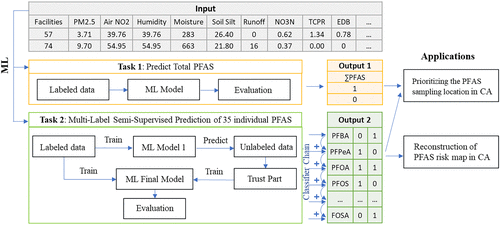
\includegraphics[width=0.95\linewidth]{Chap2/images/pipeline_dong.png}
    \caption{Pipeline bi-t\^ache de Dong et al.~\cite{dong2024pfas}. La t\^ache~1 (criblage total) repose sur une for\^et al\'eatoire avec sur-\'echantillonnage ADASYN~; la t\^ache~2 (pr\'ediction des 35 analytes) encha\^ine un pseudo-\'etiquetage semi-supervis\'e et une cha\^ine de classifieurs XGBoost. Les 112 variables contextuelles constituent l'unique entr\'ee, sans aucune concentration PFAS mesur\'ee.}
    \label{fig:dong-pipeline}
\end{figure}

Les deux t\^aches partagent le m\^eme vecteur de variables contextuelles~: la t\^ache~2 l'enrichit des seules \'etiquettes pr\'edites par la cha\^ine, jamais de concentrations mesur\'ees, ce qui maintient l'ensemble du dispositif dans le r\'egime pr\'edictif (section~\ref{sec:chap2-modes}).

% =========================================================
\mySection{Discussion}{}
\label{sec:chap2-discussion}
% =========================================================

\mySubSection{Tableau comparatif synth\'etique}{}
\label{sec:chap2-tableau}

Le tableau~\ref{tab:chap2-comparatif} synth\'etise les travaux examin\'es selon leur mode d'\'evaluation dominant, leur t\^ache et leurs m\'etriques.

\begin{table}[h!]
    \centering
    \caption{Synth\`ese comparative des approches de pr\'ediction PFAS examin\'ees. Les m\'etriques proviennent des articles sources~; protocoles et corpus diff\`erent entre \'etudes. $^*$~: pr\'esence de concentrations PFAS ou de signatures chimiques mesur\'ees dans les features.}
    \label{tab:chap2-comparatif}
    \small
    \begin{tabular}{p{2.6cm}p{2.8cm}p{2.4cm}p{1.6cm}p{2.6cm}}
        \hline
        R\'ef\'erence & M\'ethode & M\'etrique & Mode & T\^ache \\
        \hline
        Li et al.~\cite{li2022pfas} & R\'eseaux bay\'esiens & ROC-AUC $\approx 0{,}78$--$0{,}96$ & Mixte & PFAS ch. courte (MN) \\
        Hu et al.~\cite{hu2021privatewells} & Stats. contextuelles & (cartes) & Pr\'edictif pur & Vuln. puits priv\'es \\
        McMahon et al.~\cite{mcmahon2022pfas} & BRT & (descriptif) & Descriptif & Profils r\'egionaux \\
        George \& Dixit~\cite{george2021pfas} & RF / XGBoost & F1 $\approx 0{,}96/0{,}88^*$ & Mixte$^*$ & Priorisation bin. (CA) \\
        Tokranov et al.~\cite{tokranov2024pfas} & XGBoost & (national) & Mixte$^*$ & Vuln. nationale US \\
        Kibbey et al.~\cite{kibbey2020pfas} & ML supervis\'e & Pr\'ec. $\approx 90\,\%^*$ & Diagnostique & Attribution sources \\
        D\'avila-Santiago et al.~\cite{davilasantiago2022} & ML non cibl\'e & (relatif) & Diagnostique & NTS fingerprinting \\
        Cheng et Ng~\cite{cheng2019pfas} & QSAR/DNN & ROC-AUC moy. 0{,}916 & Mol\'eculaire & Bioactivit\'e mol. \\
        Dong et al.~\cite{dong2024pfas} & Semi-sup., CC & ROC-AUC 0{,}94--0{,}99 (T1) ; 0{,}73--1{,}00 (T2) & Pr\'edictif (ctx) & 35 analytes (CA) \\
        \hline
    \end{tabular}
\end{table}

On observe que les publications affichant les meilleurs scores (F1~$> 0{,}90$) mobilisent presque syst\'ematiquement des donn\'ees analytiques PFAS dans leurs entr\'ees.
Deux travaux seulement (Hu et al.\ et Dong et al.) \'evaluent leur mod\`ele en mode pr\'edictif strict~; cette lacune de documentation n'est pas anodine~: un praticien qui lit F1~$= 0{,}96$ dans un article peut croire disposer d'un outil op\'erationnel de priorisation avant analyse, alors qu'il s'agit en r\'ealit\'e d'un outil de compl\'etude d'un profil analytique partiellement connu.
Aucune \'etude publi\'ee ne compare les deux modes sur le m\^eme corpus avec le m\^eme protocole de division par site.


\mySubSection{Lecture transversale~: convergences et enseignements}{}
\label{sec:chap2-convergences}

Trois enseignements transversaux ressortent de la lecture crois\'ee des dix travaux.

\textbf{La proximit\'e industrielle est le signal le plus robuste.}
La proximit\'e aux bases militaires, aux usines fluorochimiques et aux a\'eroports ressort en t\^ete des variables explicatives dans des contextes g\'eologiques tr\`es diff\'erents, qu'elle soit mesur\'ee par les importances SHAP (George et Dixit, Tokranov, Dong et al.) ou par les ar\^etes du r\'eseau bay\'esien (Li et al.).
Ce r\'esultat constitue un fondement solide pour la s\'election des features contextuelles.

\textbf{La compl\'ementarit\'e tabulaire/relationnelle est structurellement fond\'ee.}
L'exploitation de la structure relationnelle entre analytes am\'eliore les scores par rapport aux mod\`eles tabulaires ind\'ependants~: les cha\^ines de classifieurs de Dong et al.\ en fournissent la seule d\'emonstration publi\'ee sur les PFAS.
La structure relationnelle entre puits voisins, attendue m\'ecanistiquement (section~\ref{sec:chap2-transport}), n'a en revanche pas encore \'et\'e \'evalu\'ee dans la litt\'erature PFAS~: les features contextuelles encodent le risque statique, tandis que la topologie d'\'ecoulement, encore inexploit\'ee, encoderait la corr\'elation spatiale entre puits voisins et la proximit\'e aux sources anthropiques.

\textbf{Le mode d'\'evaluation conditionne les performances de fa\c con fondamentale.}
Les \'etudes dont les features comprennent des concentrations PFAS mesur\'ees publient des scores bien sup\'erieurs (F1~$> 0{,}90$) \`a celles qui s'appuient exclusivement sur des variables contextuelles.
Cette diff\'erence ne refl\`ete pas un surcro\^it de qualit\'e algorithmique~: elle quantifie la valeur informative des mesures de laboratoire, et ne vaut que si l'on compare strictement le m\^eme mod\`ele dans les deux modes sur un m\^eme ensemble de test.


\mySubSection{Lacunes structurelles identifi\'ees}{}
\label{sec:chap2-lacunes}

L'examen crois\'e des travaux r\'ev\`ele quatre lacunes structurelles.

\paragraph{L1 -- Structure relationnelle sous-exploit\'ee.}
La majorit\'e des \'etudes tabulaires ignore les liens entre puits voisins, panaches et sources communes.
Les graphes h\'et\'erog\`enes~\cite{hu2020hgt} comblent partiellement ce vide, mais la sensibilit\'e des performances aux choix de construction du graphe (seuil de distance pour les ar\^etes, nombre de types de n\oe uds, dimension de l'embedding) n'a pas fait l'objet d'une \'etude de sensibilit\'e syst\'ematique dans la litt\'erature publi\'ee.
La question de la sensibilit\'e au seuil de distance et au nombre de types de n\oe uds reste ouverte.

\paragraph{L2 -- Biais d'\'evaluation circulaire.}
Plusieurs publications pr\'esentent des scores tr\`es \'elev\'es (F1~$> 0{,}90$) sans pr\'eciser si des concentrations PFAS mesur\'ees figurent dans les features~\cite{george2021pfas}.
Peu de travaux documentent simultan\'ement les deux modes sur le m\^eme corpus~; aucune \'etude publi\'ee ne compare les deux modes avec le m\^eme protocole de division strictement par site.
La v\'erification de l'absence de fuite d'information entre variables contextuelles et concentrations PFAS est une \'etape m\'ethodologique souvent omise.

\paragraph{L3 -- Transf\'erabilit\'e g\'eographique non valid\'ee.}
Les mod\`eles sont entra\^in\'es et test\'es sur une seule r\'egion (Californie, Minnesota, est des \'Etats-Unis).
Les validations crois\'ees spatiales (entra\^inement sur un aquif\`ere, test sur un autre de lithologie diff\'erente) restent pratiquement absentes.
Pour les graphes h\'et\'erog\`enes, la question est architecturalement profonde~: le graphe \'etant construit sur les n\oe uds d'entra\^inement, une approche inductive~\cite{hamilton2017inductive} (GraphSAGE) serait requise pour g\'en\'eraliser \`a des n\oe uds non vus.

\paragraph{L4 -- Interpr\'etabilit\'e insuffisamment standardis\'ee.}
Si SHAP~\cite{lundberg2017shap} s'impose progressivement comme standard, les protocoles varient fortement entre \'etudes.
Les pipelines hybrides graphe et boosting soul\`event des questions sp\'ecifiques non encore codifi\'ees~: comment interpr\'eter la contribution d'un embedding HGT agr\'egeant l'information de dizaines de n\oe uds voisins~? Comment comparer des valeurs TreeSHAP exactes (XGBoost, LightGBM) \`a des estimations SHAP Kernel approximatives (HGT)~? Une variable tabulaire fortement corr\'el\'ee \`a $\texttt{HGT\_emb\_0}$ verra sa valeur SHAP individuelle r\'eduite par interaction, rendant son importance marginale sous-estim\'ee.

\paragraph{Remarque sur le p\'erim\`etre g\'eographique de la revue.}
L'ensemble des travaux examin\'es porte sur des aquif\`eres nord-am\'ericains~; aucune \'etude comparable mobilisant l'apprentissage automatique sur des donn\'ees PFAS europ\'eennes ou africaines n'a \'et\'e identifi\'ee dans la litt\'erature publi\'ee.
Cette limitation intrins\`eque de la revue m\'erite d'\^etre signal\'ee~: les enseignements sur les variables pr\'edictives et les architectures restent transposables, mais les seuils r\'eglementaires (directive~UE~2020/2184~\cite{eu2020drinkingwater} vs EPA 2023~\cite{epa2023npdwr}), les contextes g\'eologiques et les pratiques de surveillance diff\`erent sensiblement.

Le tableau~\ref{tab:synthese-positionnement} positionne les principales contributions au regard de ces quatre lacunes.

\begin{table}[h!]
    \centering
    \caption{Positionnement des principales contributions au regard des quatre lacunes identifi\'ees. $\bullet$~: lacune adress\'ee~; $\circ$~: partiellement adress\'ee~; $\times$~: non adress\'ee. L1~: structure relationnelle~; L2~: biais confirmatoire~; L3~: transfert g\'eographique~; L4~: interpr\'etabilit\'e standardis\'ee.}
    \label{tab:synthese-positionnement}
    \small
    \begin{tabular}{lcccc}
        \hline
        R\'ef\'erence & L1 & L2 & L3 & L4 \\
        \hline
        Li et al.~\cite{li2022pfas}            & $\times$ & $\circ$ & $\times$ & $\times$ \\
        George et Dixit~\cite{george2021pfas}  & $\times$ & $\times$ & $\times$ & $\circ$ \\
        McMahon et al.~\cite{mcmahon2022pfas}  & $\times$ & $\circ$ & $\circ$  & $\times$ \\
        Tokranov et al.~\cite{tokranov2024pfas} & $\times$ & $\circ$ & $\bullet$ & $\circ$ \\
        Dong et al.~\cite{dong2024pfas}        & $\times$ & $\times$ & $\times$ & $\circ$ \\
        \hline
    \end{tabular}
\end{table}

Aucun travail de la litt\'erature n'adresse simultan\'ement L1, L2 et L4~: les \'etudes tabulaires ignorent la structure relationnelle~; celles qui exploitent un graphe ne documentent pas le mode pr\'edictif strict~; l'interpr\'etabilit\'e reste non standardis\'ee.
La combinaison de ces lacunes, en particulier la validation inter-aquif\`eres (L3), d\'efinit autant de directions de recherche encore ouvertes.


% =========================================================
\mySection{Synth\`ese}{}
\label{sec:synthese-chap2}
% =========================================================

Ce chapitre a dress\'e un panorama structur\'e de l'application de l'intelligence artificielle \`a la pr\'ediction et \`a la surveillance des PFAS en eaux souterraines.
La premi\`ere g\'en\'eration (mod\`eles probabilistes et arbres d'ensemble) a \'etabli le socle des variables pr\'edictives (proximit\'e aux sources, indicateurs hydrog\'eologiques, co-contaminants) et d\'emontr\'e la faisabilit\'e de la priorisation r\'egionale et nationale.
La deuxi\`eme (r\'eseaux de neurones, puis cha\^ines semi-supervis\'ees multi-\'etiquettes) a \'etendu le champ \`a plusieurs dizaines d'analytes et exploit\'e les donn\'ees non \'etiquet\'ees, sans toujours expliciter le r\'egime d'\'evaluation retenu.

Les lacunes L1--L4 dessinent en creux un syst\`eme id\'eal de priorisation~: fonctionnant sans mesure PFAS pr\'ealable (mode pr\'edictif pur), int\'egrant les relations spatiales par un graphe h\'et\'erog\`ene, interpr\'etable par SHAP globale et locale, et valid\'e sur une division spatiale ind\'ependante.
Aucune \'etude publi\'ee ne satisfait simultan\'ement ces crit\`eres.
